\documentclass[tikz,border=8pt]{standalone}
\usepackage[utf8]{inputenc}
\usepackage[T1]{fontenc}
\usepackage{lmodern}
\usetikzlibrary{arrows.meta,positioning,fit}
\definecolor{navy}{HTML}{15324B}
\definecolor{blue}{HTML}{2F80C1}
\definecolor{cyan}{HTML}{DCEFF7}
\definecolor{orange}{HTML}{E8873A}
\definecolor{green}{HTML}{3B8F72}
\tikzset{box/.style={draw=navy,rounded corners=3pt,very thick,align=center,minimum width=2.5cm,minimum height=1.15cm,fill=white,font=\sffamily},arr/.style={-{Latex[length=3mm]},very thick,navy}}
\begin{document}
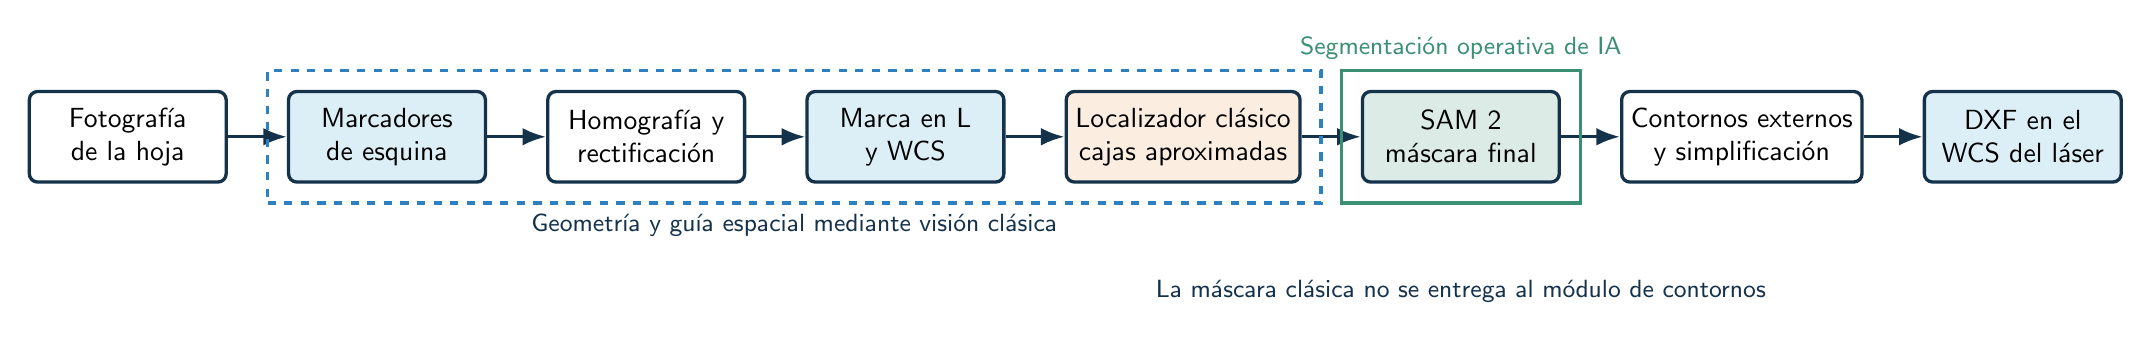
\begin{tikzpicture}[node distance=0.75cm and 0.75cm]
\node[box] (capture) {Fotografía\\de la hoja};
\node[box,right=of capture,fill=cyan] (markers) {Marcadores\\de esquina};
\node[box,right=of markers] (homography) {Homografía y\\rectificación};
\node[box,right=of homography,fill=cyan] (wcs) {Marca en L\\y WCS};
\node[box,right=of wcs,fill=orange!15] (localizer) {Localizador clásico\\cajas aproximadas};
\node[box,right=of localizer,fill=green!18] (sam) {SAM 2\\máscara final};
\node[box,right=of sam] (contours) {Contornos externos\\y simplificación};
\node[box,right=of contours,fill=cyan] (dxf) {DXF en el\\WCS del láser};
\draw[arr] (capture)--(markers); \draw[arr] (markers)--(homography); \draw[arr] (homography)--(wcs); \draw[arr] (wcs)--(localizer); \draw[arr] (localizer)--(sam); \draw[arr] (sam)--(contours); \draw[arr] (contours)--(dxf);
\node[draw=blue,dashed,very thick,fit=(markers)(homography)(wcs)(localizer),inner sep=7pt,label={[navy,font=\sffamily\small]below:Geometría y guía espacial mediante visión clásica}] {};
\node[draw=green,very thick,fit=(sam),inner sep=7pt,label={[green,font=\sffamily\small]above:Segmentación operativa de IA}] {};
\node[navy,font=\sffamily\small,align=center,below=1.1cm of sam] {La máscara clásica no se entrega al módulo de contornos};
\end{tikzpicture}
\end{document}
